%% MANUALE DELL'APPLICAZIONE
\section{Introduzione}
\subsection{Cos'è Monolith SDK?}
Monolith SDK è un pacchetto \glossario{Meteor} che consente la creazione di bolle interattive in ambiente \glossario{Rocket.chat}.\\
Lo sviluppatore avrà la possibilità di usare i componenti della SDK per costruire le proprie bolle da integrare a quelle già esistenti sulla piattaforma di \glossario{Rocket.chat}.
\subsection{Scopo del documento}
Questo documento rappresenta il manuale utente per l'applicazione Monolith SDK nel quale vengono descritte dettagliatamente tutte le caratteristiche dell'applicativo utilizzabili dallo sviluppatore.
Il manuale sarà diviso in sezioni per essere maggiormente comprensibile e spiegherà le varie feature che lo sviluppatore potrà utilizzare per costruire la propria bolla.
\subsection{Organizzazione dei repository}
Vengono forniti 4 repository:
\begin{itemize}
	\item \textbf{monolith-sdk} \\
	Contiene il codice per l'SDK. Sono fornite le funzionalità di Monolith. Tutti gli altri pacchetti dipendono da questo. \\
	\url{https://github.com/ObelixSWE/monolith-sdk}
	\item \textbf{monolith-hellobubble} \\
	Contiene il codice per l'esempio più semplice possibile su come usare l'SDK Monolith. \\
	\url{https://github.com/ObelixSWE/monolith-hellobubble}
	\item \textbf{monolith-demo} \\
	Contiene il codice per la demo ufficiale di Monolith. Rappresenta un caso d'uso più complesso rispetto a monolith-hello. Vedere la descrizione per maggiori dettagli. \\
	\url{https://github.com/ObelixSWE/monolith-demo}
	\item \textbf{monolith-emptybubble} \\
	Contiene il codice per la bolla vuota. Contiene i file che si possono usare come base per costruire la propria bolla. Vedere la guida allo sviluppo per maggiori dettagli. \\
	\url{https://github.com/ObelixSWE/monolith-emptybubble}
\end{itemize}

\subsection{Comunicazione dei bug}
Nel caso si riscontrino degli errori o dei problemi durante il normale utilizzo dell'applicazione si prega di comunicarlo al team di sviluppo aprendo un issue sul nostro repository Github:
\url{https://github.com/ObelixSWE/monolith-sdk/issues} \\
Il team si impegna a lavorare per migliorare l'applicazione e per risolvere qualunque bug venga segnalato.

\section{Requisiti per l'installazione e l'utilizzo}
\subsection{Installazione}
Monolith è stato realizzato e testato su Meteor v1.5.1 e Rocket.chat v0.59. Non si garantisce il funzionamento per versioni precedenti.
\subsection{Utilizzo}
L'esecuzione lato client è supportata sui seguenti browsers:
\begin{itemize}
	\item Google Chrome v59+
	\item Firefox v54+
	\item Internet Explorer v11+
	\item Safari v10+
\end{itemize}
Come per qualunque applicazione Meteor il browser deve avere JavaScript attivato.

\section{Installazione}
\subsection{Installazione dell'SDK}
Per installare Monolith SDK su Rocket.chat è necessario eseguire i seguenti passi:
\begin{lstlisting}
  git clone https://github.com/RocketChat/Rocket.Chat.git
  cd Rocket.Chat
  meteor npm start # al termine chiudere meteor
  meteor add templating blaze-html-templates 
		react-meteor-data maxharris9:classnames
		react-template-helper	
  meteor npm i react react-dom bluebird simple-schema 
  		react-addons-pure-render-mixin money 
  		request request-promise  --save
  # copiare monolith-sdk all'interno di Rocket.chat/packages
  # eseguire nella directory principale di Rocket.chat:
  meteor add monolith-sdk
  meteor
\end{lstlisting}

\subsection{Installazione di monolith-hello}
\textbf{Prerequisito}: monolith-sdk deve essere già installato come spiegato in \S 2.1. \\
Per installare monolith-hello su Rocket.chat è necessario eseguire i seguenti passi: 

\begin{lstlisting}
# scaricare il contenuto del repository monolith-hello e 
# inserire la directory all'interno di Rocket.chat/packages
# eseguire nella directory principale di Rocket.chat:
meteor add monolith-hello
\end{lstlisting}


\subsection{Installazione di monolith-demo}
\textbf{Prerequisito}: monolith-sdk deve essere già installato come spiegato in \S 2.1. \\
Per installare monolith-demo su Rocket.chat è necessario eseguire i seguenti passi: 

\begin{lstlisting}
# scaricare il contenuto del repository monolith-demo e 
# inserire la directory all'interno di Rocket.chat/packages
# eseguire nella directory principale di Rocket.chat:
meteor add monolith-demo
\end{lstlisting}


\section[Come creare una bolla]{Utilizzo dell'SDK per la creazione di una bolla}

\subsection{La bolla vuota come punto di partenza}
Viene fornito monolith-emptybubble come punto di partenza per lo sviluppo di una nuova bolla. La prima cosa da fare è scegliere un nome per la bolla. Da adesso sarà usato <yourbubble> per indicare il nuovo progetto. Dopo aver scaricato la directory modificare i file come segue:
\begin{itemize}
	\item Rinominare la directory principale e tutti i file utilizzando <yourbubble>
	\item \textbf{package.js}
		\begin{itemize}
			\item Cambiare il nome del package  in <yourbubble> in Package.describe name.
			\item Rinominare i files all'interno di api.addFiles. 
		\end{itemize}
	\item \textbf{client/main.js}: correggere il percorso del file.
	\item \textbf{server/main.js}: correggere il percorso del file.
	\item \textbf{server/Methods.js}: scrivere i Meteor.Method. \'E richiesto per la modifica, ma è opzionale per l'inserimento. L'utilizzo viene spiegato in \S 4.4.
	\item \textbf{lib/emptyDb.js}: rinominare la collezione utilizzando <yourbubble>.
	\item \textbf{lib/emptyCheck.js}: rinominare l'oggetto check e inserire lo schema dei dati come descritto in \S 4.3.
	\item \textbf{lib/emptyBubble.jsx}: Componente grafico. Vedere \S 4.2 per maggiori dettagli.
	\item \textbf{lib/emptyBubbleConfig.jsx}: Componente grafico. Vedere \S 4.2 per maggiori dettagli.	
	\item \textbf{lib/emptyBubbleCreationButton.jsx}: Componente grafico. Vedere \S 4.2 per maggiori dettagli.
	\item \textbf{lib/emptyCreator.jsx}: sostituire <yourbubble> al posto di empty.
		
\end{itemize}

\subsection{Componenti grafici essenziali}
Questi sono i componenti essenziali che devono essere realizzati. \'E possibile semplificare il lavoro utilizzando i componenti grafici forniti con l'SDK.

\subsubsection{emptyBubble.jsx}
\'E possibile realizzare due versioni di questo componente, per il mittente e per il ricevente, oppure usarne una come nell'esempio. Basta modificare <yourbubble>Creator.js.

Deve essere realizzato un componente React che dovrà ricevere nelle props tutti i dati della bolla per la persistenza. Se è necessario, è possibile modificare lo stato della bolla sul server utilizzando <yourbubble>Db.

\subsubsection{emptyBubbleConfig.jsx}
Deve essere realizzato un componente React che dovrà ricevere nelle props una funzione \emph{closeMenu}. Utilizzare la funzione per chiudere il menu quando la configurazione della bolla è terminata, come nell'esempio:

\begin{lstlisting}
send(){
	let insProm = <yourbubble>Db.insert({...});
	insProm.then(
		(result) => {this.props.closeMenu();},
		(error) => {console.log(error);}
	);
}
\end{lstlisting}

L'esempio usa la sintassi delle promise. Se l'operazione viene eseguita il menu si chiude. 

Per inserire la bolla nel database lato server bisogna usare <yourbubble>Db.

\subsubsection{emptyBubbleCreationButton.jsx}
Questo componente rappresenta il pulsante nel menu per cominciare la configurazione di <yourbubble>. Per un utilizzo di base basta semplicemente inserire <yourbubble> nel file dato.

Se sono necessari due pulsanti (come in monolith-demo) è possibile ridefinire il metodo \emph{secondAreaName}. Bisogna anche passare come props \emph{secondButtonName}. Si noti che sarà necessario un secondo configmenu e un creator
rinominati di conseguenza.

\subsection{Descrizione dello schema dei dati}
In <yourbubble>Check.js è necessario definire uno schema per validare i dati da inserire nel database. Definire lo schema usando la sintassi SimpleSchema: \url{https://www.npmjs.com/package/simpl-schema}

\subsection{Configurazione del database e possibili usi}

In <yourbubble>Db.js basta semplicemente inserire il nome corretto per la propria bolla. In <yourbubble>Methods.js è possibile inserire i metodi Meteor da chiamare per l'inserimento o la modifica della bolla:

\subsubsection{Metodi per l'inserimento}
\emph{L'uso è opzionale}. 
\begin{lstlisting}
newDataObj method(dataObj);
\end{lstlisting}

Viene modificato l'oggetto dei dati inviato dal client prima di essere controllato. Si noti che l'oggetto modificato deve essere restituito. \'E possibile chiamare il metodo inserendo il nome del metodo come argomento di <yourbubble>Db.

\subsubsection{Metodi per la modifica}
\emph{L'uso è obbligatorio}. 
\begin{lstlisting}
boolean method(bubbleId, argument);
\end{lstlisting}

In questo metodo è necessario inserire tutte le operazioni di modifica del database per <yourbubble>. Deve restituire true in caso di successo, false in caso di fallimento. \'E possibile chiamare il metodo  inserendo
il nome del metodo come argomento di <yourbubble>Db.

\section{Descrizione delle classi utilizzabili}
Questa sezione spiega come utilizzare le classi della libreria Monolith.

\subsection{SingleComponents}
Le classi SingleComponents rappresentano i componenti che possono essere renderizzati.
\begin{flushleft}
\subsubsection{CheckButton}
CheckButton rappresenta il tag HTML <checkbox>.
\begin{verbatim}
<CheckButton
	id="HTML id"
	classes="CSS classes"
	getCheck={this.functionName}
	value="checkbox value"
/>
\end{verbatim}
	
getCheck è una props associata a una funzione che viene chiamata quando l'evento onChange della checkbox è chiamato e passa alla funzione una variabile contenente lo stato del checkbox.

\begin{verbatim}
functionName(m){...}

m={id:"id", value:"value", check:[true/false]};
\end{verbatim}


\subsubsection{CheckBoxList}
CheckBoxList rappresenta un gruppo di CheckButton. 
CheckBoxList ha bisogno di ricevere un array come questo: 
\begin{verbatim}
let opt=[{id: 1, value: 'Hello World'},{id: 2, value: 'Installation'}];

<CheckBoxList
	classes="CSS classes"
	options={opt}
	getCheck={this.functionName}
/>
\end{verbatim}
getCheck come CheckButton getCheck.
\begin{verbatim}
functionName(m){...}

m={id:"id", value:"value", check:[true/false]};
\end{verbatim}

\begin{center}

\underline{\textit{Esempio:}}
\\
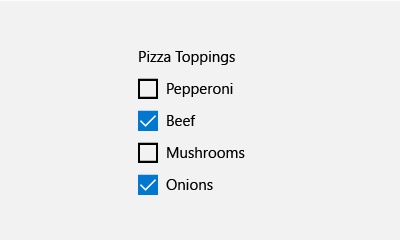
\includegraphics[scale=0.53]{img/checkbox.png}
\\
\end{center}

\subsubsection{ComboBox}
ComboBox rappresenta il tag HTML <select>.
\begin{verbatim}
<ComboBox
	id="HTML id"
	classes="CSS classes"
	options={["a","b","c"]}
	getSelection={this.functionName}
/>
\end{verbatim}

getSelection è una props associata a una funzione che viene chiamata quando l'evento onChange della select è chiamato e passa alla funzione una variabile contenente l'opzione selezionata.

\begin{verbatim}
functionName(m){...}

m="selected option";
\end{verbatim}

\begin{center}

\underline{\textit{Esempio:}}
\\
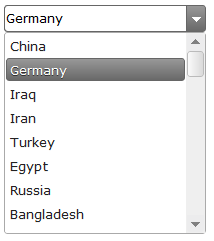
\includegraphics[scale=0.9]{img/combobox.png}

\end{center}

\subsubsection{Image}
Image rappresenta il tag HTML <img>.

\begin{verbatim}
<Image
	id="HTML id"
	classes="CSS classes"
	src="img source location"
	alt="image description"
	width="image width"
	height="image height"
/>
\end{verbatim}

\subsubsection{ImageButton}
ImageButton rappresenta un'immagine cliccabile come se fosse un pulsante.
\begin{verbatim}
<ImageButton
	id="HTML id"
	src="img source location"
	alt="image description"
	width="image width"
	height="image height"
	handleClick={this.functionName}
/>
\end{verbatim}

handleClick è una props associata a una funzione che viene chiamata quando l'ImageButton viene cliccato.

\begin{verbatim}
functionName(id){...}
id="id of the clicked button"
\end{verbatim}

\subsubsection{LineEdit}
LineEdit rappresenta il tag HTML di testo <input>.

\begin{verbatim}
<LineEdit
	id="HTML id"
	classes="CSS classes"
	updateState={this.functionName}
	value="default value"
/>
\end{verbatim}

updateState è una props associata a una funzione che viene chiamata quando l'evento onChange del text input è chiamato.

\begin{verbatim}
updateState(text,id){...}

text="text of the text input"
id="id of the text input"
\end{verbatim}

\begin{center}
\underline{\textit{Esempio:}}
\\

\includegraphics[scale=1]{img/lineedit.png}
\\
\end{center}

\subsubsection{LineEditComboBox}
LineEditComboBox rappresenta il tag HTML di testo <input> e il tag HTML <select>.
\begin{verbatim}
<LineEditComboBox
	idle="LineEdit HTML id"
	idcb="ComboBox  HTML id"
	classesle="LineEdit CSS classes"
	classescb="ComboBox CSS classes"
	textUpdate={this.functionName1}
	options={["a","b","c"]}
	comboUpdate={this.functionName2}
/>
\end{verbatim}

textUpdate è una props associata a una funzione che viene passata al LineEdit.
comboUpdate è una props associata a una funzione che viene passata al ComboBox

\begin{verbatim}
functionName1(text,id){...}

text="text of the text input"
id="id of the text input"

functionName2(m){...}

m="selected option";
\end{verbatim}

\subsubsection{PushButton}
PushButton rappresenta il tag HTML <button>.
\begin{verbatim}
<PushButton
id="HTML id"
classes="CSS classes"
handleClick={this.functionName}
buttonName="button name"
/>
\end{verbatim}
handleClick è una props associata a una funzione che viene chiamata quando il pulsante viene cliccato.
\begin{verbatim}
functionName(id){...}

id="id of the button"
\end{verbatim}


\begin{center}
	\underline{\textit{Esempio:}}
	\\
	
\includegraphics[scale=0.25]{img/pushB.png}
	\\
\end{center}

\subsubsection{LineEditPushButton}
LineEditPushButton rappresenta un LineEdit e un PushButton.
\begin{verbatim}
<LineEditPushButton
	idle="LineEdit HTML id"
	idpb="PushButton HTML id"
	classesle="LineEdit CSS classes"
	classespb="PushButton CSS classes"
	getText={this.functionName}
	buttonName="button name"
/>
\end{verbatim}
getText è una props associata a una funzione che viene chiamata quando il PushButton viene cliccato e passa alla funzione una variabile contenente il testo del LineEdit.
\begin{verbatim}
functionName(text){...}

text="text of the LineEdit"
\end{verbatim}

\begin{center}
\underline{\textit{Esempio:}}
\\
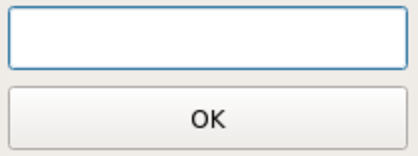
\includegraphics[scale=0.75]{img/LEPush.png}
\\
\end{center}

\subsubsection{RadioButtonGroup}
RadioButtonGroup rappresenta un gruppo di tag HTML radio button <input>.
\begin{verbatim}
<RadioButtonGroup
	classes="CSS classes"
	options={["a","b","c"]}
	getValue={this.functionName}
/>
\end{verbatim}
getValue è una props associata a una funzione che viene chiamata quando un radio button viene cliccato e passa alla funzione una variabile contenente l'informazione sul radio button selezionato.
\begin{verbatim}
functionName(value){...}

value="value of the selected radio button"
\end{verbatim}

\begin{center}
\underline{\textit{Esempio:}}
\\
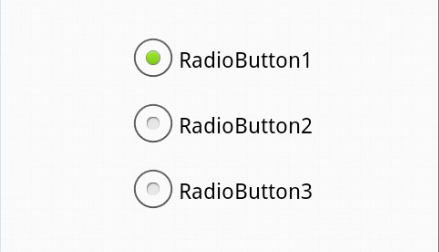
\includegraphics[scale=0.6]{img/radiob.png}
\\
\end{center}

\subsubsection{TextAreaButton}

TextAreaButton rappresenta il tag HTML <textarea> e un PushButton.
\begin{verbatim}
<TextAreaButton
	idta="textArea HTML id"
	classesta="textArea CSS classes"
	idpb="PushButton HTML id"
	classespb="PushButton CSS classes"
	getText={this.functionName}
	width="textarea width"
	height="textarea height"
	buttonName="button name"
/>
\end{verbatim}
getText è una props associata a una funzione che viene chiamata quando il PushButton viene cliccato e passa alla funzione una variabile contenente il testo della textarea.
\begin{verbatim}
functionName(text){...}

text="text of the textarea"
\end{verbatim}

\begin{center}
\underline{\textit{Esempio:}}
\\
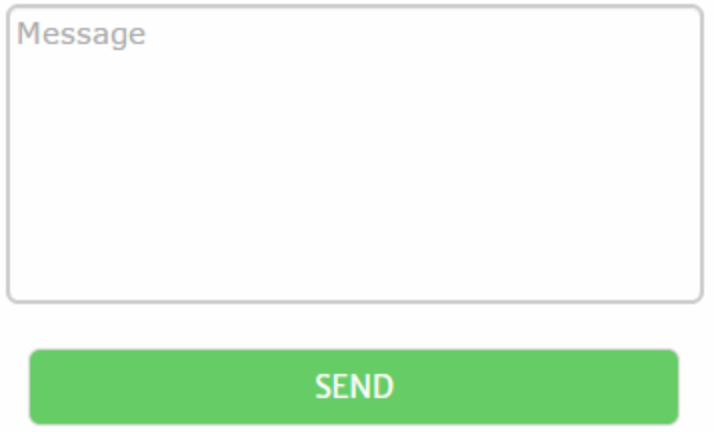
\includegraphics[scale=0.5]{img/textB.png}
\\
\end{center}

\subsubsection{TextAreaComboBox}
TextAreaComboBox rappresenta il tag HTML <textarea> e un ComboBox.
\begin{verbatim}
<TextAreaComboBox
	idtx="textArea HTML id"
	classestx="textArea CSS classes"
	idcb="combobox HTML id"
	classescb="combobox CSS classes"
	width="textarea width"
	height="textarea height"
	textUpdate={this.functionName1}
	options={["a","b","c"]}
	comboUpdate={this.functionName2}
/>
\end{verbatim}
textUpdate è una props associata a una funzione che viene chiamata quando l'evento onChange della textarea è chiamato.\\
comboUpdate è una props associata a una funzione che viene chiamata quando l'evento onChange della select  è chiamato e passa alla funzione una variabile contenente l'opzione selezionata.
\begin{verbatim}
functionName1(text){...}

text="text of the textarea"

functionName2(m){...}

m="selected option";
\end{verbatim}
\end{flushleft}

\subsection{Layout}
Layout sono classi che rappresentano contenitori che posizionano gli elementi contenuti in un certo modo.
\begin{flushleft}
\subsubsection{VerticalLayout}
VerticalLayout rappresenta un contenitore che posiziona gli elementi contenuti uno sotto l'altro. La props \textit{hide} permette di nascondere la vista del layout (tramite valori \textit{true/false}).
\begin{verbatim}
	<VerticalLayout hide={}>
	<Children/>
	<Children/>
	.
	.
	.
	</VerticalLayout>
\end{verbatim}


\subsubsection{HorizontalalLayout}
HorizontalLayout rappresenta un contenitore che posiziona gli elementi contenuti uno accanto all'altro. La props \textit{hide} permette di nascondere la vista del layout (tramite valori \textit{true/false}).

\begin{verbatim}
	<HorizontalLayout hide={}>
	<Children/>
	<Children/>
	.
	.
	.
	</HorizontalLayout>
\end{verbatim}
\end{flushleft}

\section{Utilizzo delle bolle}
Vengono fornite alcune bolle tipo che possono essere create tramite il menù apposito presente nella tabbar laterale di Rochet.chat.\\

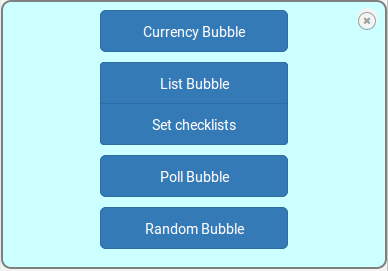
\includegraphics[scale=0.75]{img/menu.png}
\newpage
\subsection{CurrencyBubble}
La \textit{CurrencyBubble} è una bolla che funge da convertitore di valuta.
\\Una volta selezionata dal menù la si può configurare impostando la valuta di base, di uscita ed il valore da convertire.\\

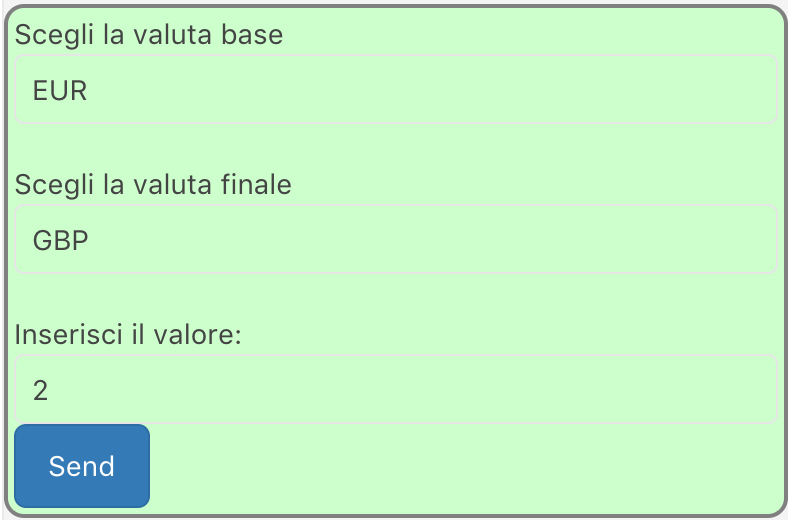
\includegraphics[scale=0.75]{img/currConfig.png}
\\
Una volta inviata cliccando su \textbf{Send} il risultato sarà:\\

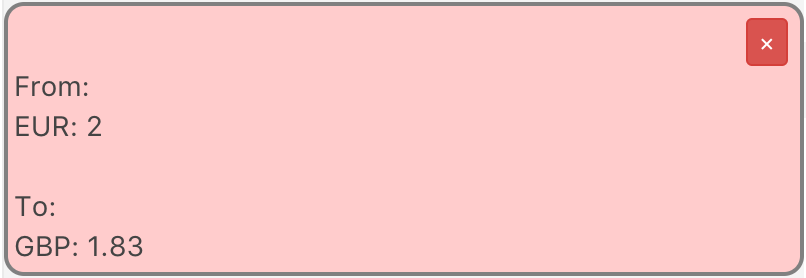
\includegraphics[scale=0.75]{img/curr.png}
\newpage
\subsection{PollBubble}
La \textit{PollBubble} è una bolla che permette di creare un sondaggio da lanciare ai membri della chat in questione.\\
Utilizzando il menù di configurazione è possibile impostare la domanda e le varie opzioni (che si possono aggiungere con il pulsante \textbf{Add}).
\\

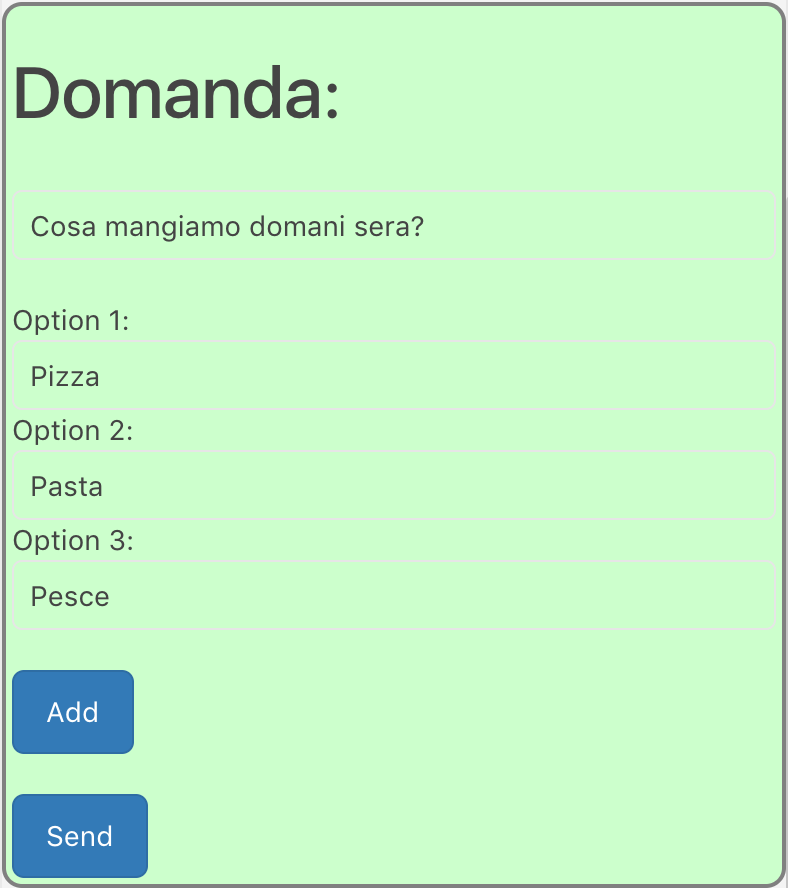
\includegraphics[scale=0.75]{img/pollConfig.png}

Una volta inviata cliccando su \textbf{Send} il risultato sarà:\\

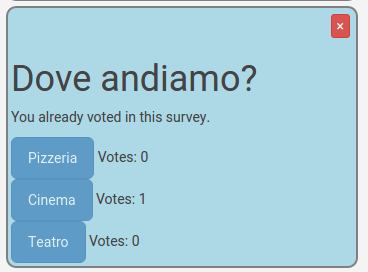
\includegraphics[scale=0.74]{img/poll.png}
\\
Dopo che la bolla è stata inviata sarà possibile votare cliccando sull'opzione desiderata. \'E possibile esprimere il voto una volta sola.
\subsection{RandomBubble}
La \textit{RandomBubble} è una bolla che lancia un certo tipo di dado (a scelta in base al numero di facce) e ne ritorna un risultato casuale.\\
Dal menù di configurazione bisognerà scegliere il numero di facce del dado.\\

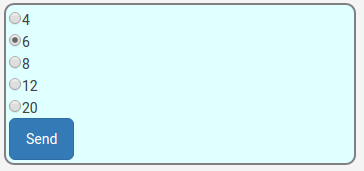
\includegraphics[scale=0.75]{img/randConfig.png}

Una volta inviata cliccando su \textbf{Send} il risultato sarà:\\

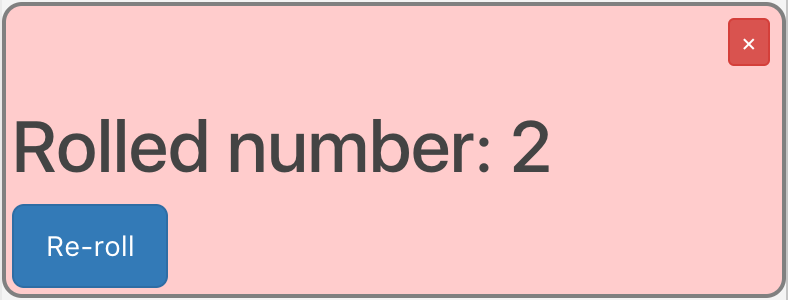
\includegraphics[scale=0.75]{img/rand.png}
\\
Attraverso il pulsante \textbf{Re-roll} si potrà rilanciare il dado.

\newpage

\section{Utilizzo della DEMO - Lista con Checklist}

\subsection{Checklist}

\begin{flushleft}
Le Checklist sono delle liste di elementi che possono essere selezionati e inseriti in altre liste.
Per creare una nuova checklist selezionare il pulsante \textbf{Set Checklist}.\\
\begin{center}
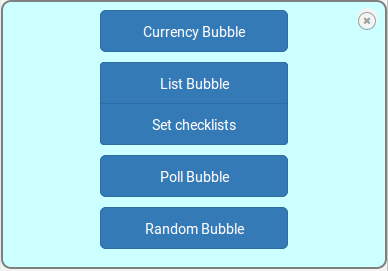
\includegraphics[scale=0.75]{img/menu.png}
\end{center}

Una volta selezionato il pulsante \textbf{Set Checklist} dal menù di creazione delle bolle si aprirà il menù di configurazione della checklist.\\
\begin{center}
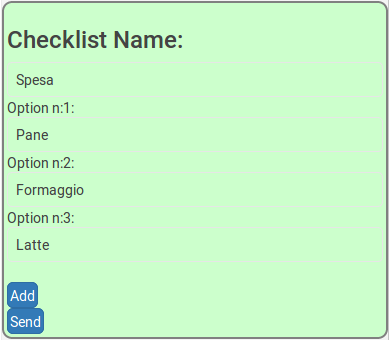
\includegraphics[scale=0.75]{img/checklist_conf.png}
\end{center}

Nel menù di configurazione bisogna inserire il nome della checklist e uno o più elementi.
Per aggiungere un' opzione bisogna selezionare il pulsante \textbf{Add}.

Una volta completata la compilazione premendo il pulsante \textbf{Send} la checklist verrà inviata al server e sarà disponibile nella creazione delle liste.
\end{flushleft}

\subsection{Lista}
\begin{flushleft}
La \textit{Lista} è una bolla che permette di creare una lista nella quale è possibile aggiungere degli elementi prelevandoli dalle checklist precedentemente definite o inserendoli manualmente.

Per creare una nuova lista selezionare il pulsante \textbf{ListBubble} dal menù di creazione delle bolle.\\
\begin{center}
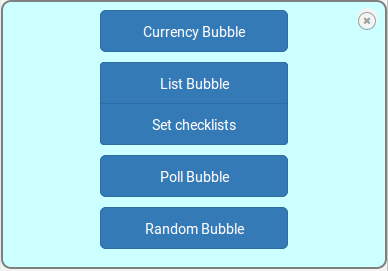
\includegraphics[scale=0.75]{img/menu.png}
\end{center}
\newpage
Una volta selezionato il pulsante \textbf{ListBubble} si aprirà il menù di configurazione della lista.\\
\begin{center}
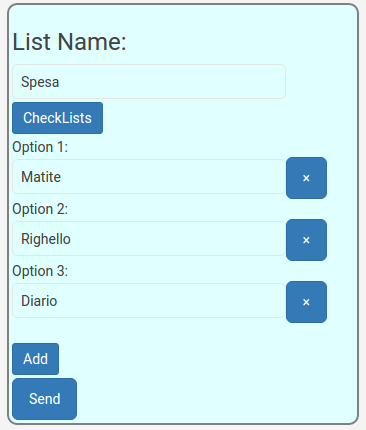
\includegraphics[scale=0.75]{img/list_conf.png}
\end{center}

Nel menù di configurazione bisogna inserire il nome della lista e una o più opzioni.
Per aggiungere una opzione bisogna selezionare il pulsante \textbf{Add} oppure si possono prelevare gli elementi dalla lista delle checklist.
Per aprire il menù di selezione delle checklist bisogna premere il pulsante \textbf{Checklists} nel menù di configurazione della lista.\\
\begin{center}
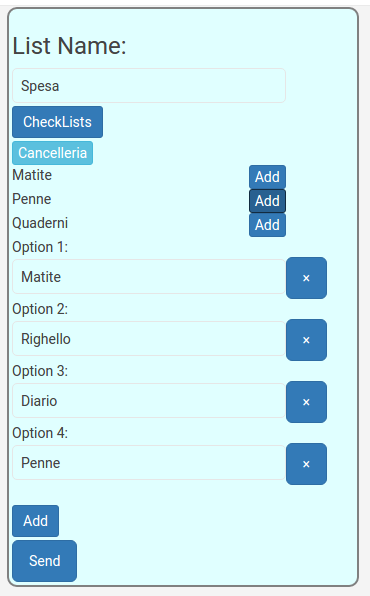
\includegraphics[scale=0.75]{img/list_checklist1.png}
\end{center}

Premendolo nuovamente il menù delle checklist verrà chiuso.
Una volta selezionate le checklist bisogna premere il pulsante \textbf{Add checklist} per aggiungerle alla lista.\\
\begin{center}
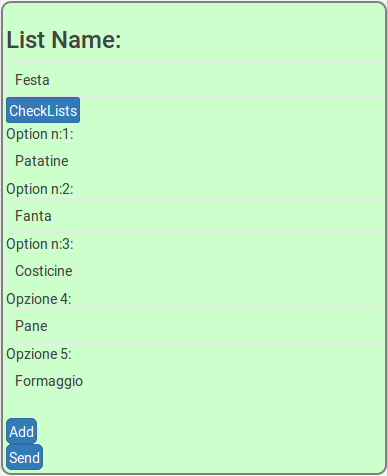
\includegraphics[scale=0.65]{img/list_checklist2.png}
\end{center}

Una volta completata la compilazione premendo il pulsante \textbf{Send} la lista verrà inviata al server e sarà visualizza nell'area contenente le bolle inviate.

\begin{center}
	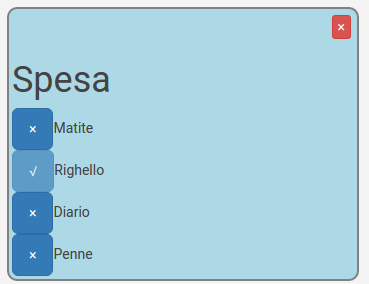
\includegraphics[scale=0.70]{img/list_checklist.png}
\end{center}

\'E possibile spuntare gli elementi della lista.

\end{flushleft}

\newpage

\appendix
\setcounter{secnumdepth}{0}
\section{Glossario}

\subsection*{B}
\begin{itemize}
\item 
\textbf{Bolla}: messaggio che può essere inviato all'interno della chat. Aggiunge alle funzionalità base della chat, nuove funzionalità che sono accessibili direttamente dalla conversazione senza il bisogno di ricorrere all'apertura di applicazioni diverse.
\item
\textbf{Bug}: Il termine inglese bug, in italiano baco, identifica in informatica un errore nella scrittura del codice sorgente di un programma software. Meno comunemente, il termine bug può indicare un difetto di progettazione in un componente hardware, che ne causa un comportamento imprevisto o comunque diverso da quello specificato dal produttore.
\end{itemize}
\newpage

\subsection*{D}
\begin{itemize}
\item
\textbf{Demo}: il demo (abbreviazione dell'inglese demonstration, che significa prova, dimostrazione) è un campione dimostrativo della produzione di musicisti, scrittori, programmatori e autori in genere. \'E prodotto e distribuito dallo stesso autore o da suoi produttori/agenti, solitamente in maniera gratuita, allo scopo di promuovere l'autore presso enti in grado di operare una distribuzione/produzione di più ampio raggio (case editrici, case discografiche, aziende produttrici e così via).
\end{itemize}
\newpage

\subsection*{G}
\begin{itemize}
	\item
    \textbf{Git}: è un software di controllo versione distribuito utilizzabile da interfaccia a riga di comando, creato da Linus Torvalds nel 2005.
	\item
	\textbf{Github}: è un servizio di hosting per progetti software. Il nome deriva dal fatto che GitHub è un servizio sostitutivo del software dell'omonimo strumento di controllo versione distribuito, Git.
\end{itemize}
\newpage

\subsection*{M}
\begin{itemize}
	\item
	\textbf{Meteor}: Meteor, or MeteorJS, is a free and open-source JavaScript web framework written using Node.js. Meteor allows for rapid prototyping and produces cross-platform (Android, iOS, Web) code. It integrates with MongoDB and uses the Distributed Data Protocol and a publish-subscribe pattern to automatically propagate data changes to clients without requiring the developer to write any synchronization code. On the client, Meteor depends on jQuery and can be used with any JavaScript UI widget library.
	\item
	\textbf{Monolith}: Monolith is an open source Rocket.chat library developed by NPE Developers which helps Meteor developers to build interactive bubbles.
\end{itemize}
\newpage

\subsection*{R}
\begin{itemize}
	\item
    \textbf{React}: è una libreria Javascript open source che permette di costruire interfacce utente.
    \item
    \textbf{Repository}: un repository (letteralmente deposito o ripostiglio) è un ambiente di un sistema informativo (ad es. di tipo ERP), in cui vengono gestiti i metadati.
	\item
	\textbf{Rocket.Chat}: web chat open source. Sistema che permette agli utenti di comunicare in tempo reale utilizzando interfacce web facilmente accessibili.
\end{itemize}
\newpage

\subsection*{S}
\begin{itemize}
	\item
	\textbf{SDK}: software development kit (SDK, traducibile in italiano come "pacchetto di sviluppo per applicazioni"), in informatica, indica genericamente un insieme di strumenti per lo sviluppo e la documentazione di software. Nel contesto del progetto indica tutto Monolith a parte le bolle d'esempio e la Demo.
	\item
    \textbf{sidearea}: per sidearea si intende una delle due aree che Monolith crea in Rocket.Chat alla pressione dei pulsanti nella tabbar. Si tratta di una parte dello schermo sulla destra che diventa fullscreen in visualizzazione mobile.
\end{itemize}
\newpage

\subsection*{T}
\begin{itemize}
\item
\textbf{tabbar}: in Rocket.Chat è la parte della finestra di chat più a destra su cui si trovano alcuni pulsanti. \'E qui che Monolith aggiunge i suoi pulsanti.
\end{itemize}
\newpage

\subsection*{W}
\begin{itemize}
\item
\textbf{Webapp}: in informatica l'espressione applicazione web, ovvero web-application in inglese, indica genericamente tutte le applicazioni distribuite web-based. Nell'ingegneria del software e nella programmazione Web essa indica infatti un'applicazione accessibile/fruibile via web per mezzo di un network, come ad esempio una Intranet all'interno di un sistema informatico o attraverso la Rete Internet, ovvero in una architettura tipica di tipo client-server, che offre determinati servizi all'utente client
\end{itemize}
\newpage
